\documentclass[1p]{elsarticle_modified}
%\bibliographystyle{elsarticle-num}

%\usepackage[colorlinks]{hyperref}
%\usepackage{abbrmath_seonhwa} %\Abb, \Ascr, \Acal ,\Abf, \Afrak
\usepackage{amsfonts}
\usepackage{amssymb}
\usepackage{amsmath}
\usepackage{amsthm}
\usepackage{scalefnt}
\usepackage{amsbsy}
\usepackage{kotex}
\usepackage{caption}
\usepackage{subfig}
\usepackage{color}
\usepackage{graphicx}
\usepackage{xcolor} %% white, black, red, green, blue, cyan, magenta, yellow
\usepackage{float}
\usepackage{setspace}
\usepackage{hyperref}

\usepackage{tikz}
\usetikzlibrary{arrows}

\usepackage{multirow}
\usepackage{array} % fixed length table
\usepackage{hhline}

%%%%%%%%%%%%%%%%%%%%%
\makeatletter
\renewcommand*\env@matrix[1][\arraystretch]{%
	\edef\arraystretch{#1}%
	\hskip -\arraycolsep
	\let\@ifnextchar\new@ifnextchar
	\array{*\c@MaxMatrixCols c}}
\makeatother %https://tex.stackexchange.com/questions/14071/how-can-i-increase-the-line-spacing-in-a-matrix
%%%%%%%%%%%%%%%

\usepackage[normalem]{ulem}

\newcommand{\msout}[1]{\ifmmode\text{\sout{\ensuremath{#1}}}\else\sout{#1}\fi}
%SOURCE: \msout is \stkout macro in https://tex.stackexchange.com/questions/20609/strikeout-in-math-mode

\newcommand{\cancel}[1]{
	\ifmmode
	{\color{red}\msout{#1}}
	\else
	{\color{red}\sout{#1}}
	\fi
}

\newcommand{\add}[1]{
	{\color{blue}\uwave{#1}}
}

\newcommand{\replace}[2]{
	\ifmmode
	{\color{red}\msout{#1}}{\color{blue}\uwave{#2}}
	\else
	{\color{red}\sout{#1}}{\color{blue}\uwave{#2}}
	\fi
}

\newcommand{\Sol}{\mathcal{S}} %segment
\newcommand{\D}{D} %diagram
\newcommand{\A}{\mathcal{A}} %arc


%%%%%%%%%%%%%%%%%%%%%%%%%%%%%5 test

\def\sl{\operatorname{\textup{SL}}(2,\Cbb)}
\def\psl{\operatorname{\textup{PSL}}(2,\Cbb)}
\def\quan{\mkern 1mu \triangleright \mkern 1mu}

\theoremstyle{definition}
\newtheorem{thm}{Theorem}[section]
\newtheorem{prop}[thm]{Proposition}
\newtheorem{lem}[thm]{Lemma}
\newtheorem{ques}[thm]{Question}
\newtheorem{cor}[thm]{Corollary}
\newtheorem{defn}[thm]{Definition}
\newtheorem{exam}[thm]{Example}
\newtheorem{rmk}[thm]{Remark}
\newtheorem{alg}[thm]{Algorithm}

\newcommand{\I}{\sqrt{-1}}
\begin{document}

%\begin{frontmatter}
%
%\title{Boundary parabolic representations of knots up to 8 crossings}
%
%%% Group authors per affiliation:
%\author{Yunhi Cho} 
%\address{Department of Mathematics, University of Seoul, Seoul, Korea}
%\ead{yhcho@uos.ac.kr}
%
%
%\author{Seonhwa Kim} %\fnref{s_kim}}
%\address{Center for Geometry and Physics, Institute for Basic Science, Pohang, 37673, Korea}
%\ead{ryeona17@ibs.re.kr}
%
%\author{Hyuk Kim}
%\address{Department of Mathematical Sciences, Seoul National University, Seoul 08826, Korea}
%\ead{hyukkim@snu.ac.kr}
%
%\author{Seokbeom Yoon}
%\address{Department of Mathematical Sciences, Seoul National University, Seoul, 08826,  Korea}
%\ead{sbyoon15@snu.ac.kr}
%
%\begin{abstract}
%We find all boundary parabolic representation of knots up to 8 crossings.
%
%\end{abstract}
%\begin{keyword}
%    \MSC[2010] 57M25 
%\end{keyword}
%
%\end{frontmatter}

%\linenumbers
%\tableofcontents
%
\newcommand\colored[1]{\textcolor{white}{\rule[-0.35ex]{0.8em}{1.4ex}}\kern-0.8em\color{red} #1}%
%\newcommand\colored[1]{\textcolor{white}{ #1}\kern-2.17ex	\textcolor{white}{ #1}\kern-1.81ex	\textcolor{white}{ #1}\kern-2.15ex\color{red}#1	}

{\Large $\underline{12n_{0628}~(K12n_{0628})}$}

\setlength{\tabcolsep}{10pt}
\renewcommand{\arraystretch}{1.6}
\vspace{1cm}\begin{tabular}{m{100pt}>{\centering\arraybackslash}m{274pt}}
\multirow{5}{120pt}{
	\centering
	\includegraphics[width=112pt]{../../../GIT/diagram.site/Diagrams/png/2717_12n_0628.png}\\
\ \ \ A knot diagram\footnotemark}&
\allowdisplaybreaks
\textbf{Linearized knot diagam} \\
\cline{2-2}
 &
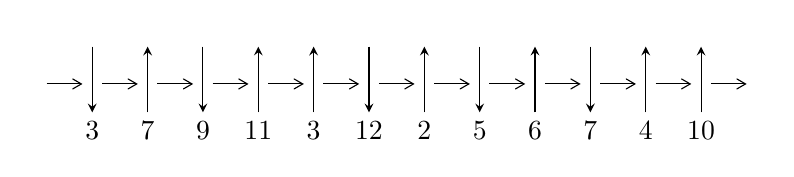
\begin{tikzpicture}[x=20pt, y=17pt]
	% nodes
	\node (C0) at (0, 0) {};
	\node (C1) at (1, 0) {};
	\node (C1U) at (1, +1) {};
	\node (C1D) at (1, -1) {3};

	\node (C2) at (2, 0) {};
	\node (C2U) at (2, +1) {};
	\node (C2D) at (2, -1) {7};

	\node (C3) at (3, 0) {};
	\node (C3U) at (3, +1) {};
	\node (C3D) at (3, -1) {9};

	\node (C4) at (4, 0) {};
	\node (C4U) at (4, +1) {};
	\node (C4D) at (4, -1) {11};

	\node (C5) at (5, 0) {};
	\node (C5U) at (5, +1) {};
	\node (C5D) at (5, -1) {3};

	\node (C6) at (6, 0) {};
	\node (C6U) at (6, +1) {};
	\node (C6D) at (6, -1) {12};

	\node (C7) at (7, 0) {};
	\node (C7U) at (7, +1) {};
	\node (C7D) at (7, -1) {2};

	\node (C8) at (8, 0) {};
	\node (C8U) at (8, +1) {};
	\node (C8D) at (8, -1) {5};

	\node (C9) at (9, 0) {};
	\node (C9U) at (9, +1) {};
	\node (C9D) at (9, -1) {6};

	\node (C10) at (10, 0) {};
	\node (C10U) at (10, +1) {};
	\node (C10D) at (10, -1) {7};

	\node (C11) at (11, 0) {};
	\node (C11U) at (11, +1) {};
	\node (C11D) at (11, -1) {4};

	\node (C12) at (12, 0) {};
	\node (C12U) at (12, +1) {};
	\node (C12D) at (12, -1) {10};
	\node (C13) at (13, 0) {};

	% arrows
	\draw[->,>={angle 60}]
	(C0) edge (C1) (C1) edge (C2) (C2) edge (C3) (C3) edge (C4) (C4) edge (C5) (C5) edge (C6) (C6) edge (C7) (C7) edge (C8) (C8) edge (C9) (C9) edge (C10) (C10) edge (C11) (C11) edge (C12) (C12) edge (C13) ;	\draw[->,>=stealth]
	(C1U) edge (C1D) (C2D) edge (C2U) (C3U) edge (C3D) (C4D) edge (C4U) (C5D) edge (C5U) (C6U) edge (C6D) (C7D) edge (C7U) (C8U) edge (C8D) (C9D) edge (C9U) (C10U) edge (C10D) (C11D) edge (C11U) (C12D) edge (C12U) ;
	\end{tikzpicture} \\
\hhline{~~} \\& 
\textbf{Solving Sequence} \\ \cline{2-2} 
 &
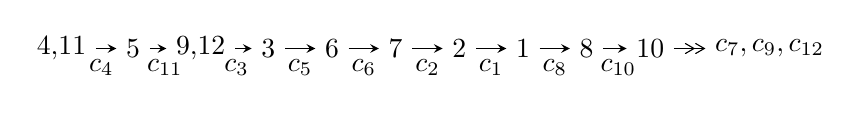
\begin{tikzpicture}[x=23pt, y=7pt]
	% node
	\node (A0) at (-1/8, 0) {4,11};
	\node (A1) at (1, 0) {5};
	\node (A2) at (33/16, 0) {9,12};
	\node (A3) at (25/8, 0) {3};
	\node (A4) at (33/8, 0) {6};
	\node (A5) at (41/8, 0) {7};
	\node (A6) at (49/8, 0) {2};
	\node (A7) at (57/8, 0) {1};
	\node (A8) at (65/8, 0) {8};
	\node (A9) at (73/8, 0) {10};
	\node (C1) at (1/2, -1) {$c_{4}$};
	\node (C2) at (3/2, -1) {$c_{11}$};
	\node (C3) at (21/8, -1) {$c_{3}$};
	\node (C4) at (29/8, -1) {$c_{5}$};
	\node (C5) at (37/8, -1) {$c_{6}$};
	\node (C6) at (45/8, -1) {$c_{2}$};
	\node (C7) at (53/8, -1) {$c_{1}$};
	\node (C8) at (61/8, -1) {$c_{8}$};
	\node (C9) at (69/8, -1) {$c_{10}$};
	\node (A10) at (11, 0) {$c_{7},c_{9},c_{12}$};

	% edge
	\draw[->,>=stealth]	
	(A0) edge (A1) (A1) edge (A2) (A2) edge (A3) (A3) edge (A4) (A4) edge (A5) (A5) edge (A6) (A6) edge (A7) (A7) edge (A8) (A8) edge (A9) ;
	\draw[->>,>={angle 60}]	
	(A9) edge (A10);
\end{tikzpicture} \\ 

\end{tabular} \\

\footnotetext{
The image of knot diagram is generated by the software ``\textbf{Draw programme}" developed by Andrew Bartholomew(\url{http://www.layer8.co.uk/maths/draw/index.htm\#Running-draw}), where we modified some parts for our purpose(\url{https://github.com/CATsTAILs/LinksPainter}).
}\phantom \\ \newline 
\centering \textbf{Ideals for irreducible components\footnotemark of $X_{\text{par}}$} 
 
\begin{align*}
I^u_{1}&=\langle 
4.23039\times10^{40} u^{36}+1.59605\times10^{41} u^{35}+\cdots+6.26742\times10^{42} b-2.10116\times10^{42},\\
\phantom{I^u_{1}}&\phantom{= \langle  }7.35912\times10^{41} u^{36}+3.34060\times10^{42} u^{35}+\cdots+5.64068\times10^{43} a+1.24742\times10^{44},\\
\phantom{I^u_{1}}&\phantom{= \langle  }u^{37}+5 u^{36}+\cdots+135 u+216\rangle \\
I^u_{2}&=\langle 
-287727135 u^{24} a-4296024791 u^{24}+\cdots+46372736648 a-5064132100,\\
\phantom{I^u_{2}}&\phantom{= \langle  }203474647775 u^{24} a+191008518002 u^{24}+\cdots+1275756399988 a+9676139674612,\\
\phantom{I^u_{2}}&\phantom{= \langle  }u^{25}-2 u^{24}+\cdots-30 u+28\rangle \\
I^u_{3}&=\langle 
-31 u^{15} a-25 u^{15}+\cdots+35 a+221,\;344 u^{15} a+659 u^{15}+\cdots+206 a+177,\;u^{16}+u^{15}+\cdots-3 u+1\rangle \\
I^u_{4}&=\langle 
u^4-2 u^3+2 u^2+b-2 u,\;u^4- u^3+a+u-2,\;u^5-2 u^4+3 u^3-3 u^2+u-1\rangle \\
\\
I^v_{1}&=\langle 
a,\;b^2- b+1,\;v+1\rangle \\
\end{align*}
\raggedright * 5 irreducible components of $\dim_{\mathbb{C}}=0$, with total 126 representations.\\
\footnotetext{All coefficients of polynomials are rational numbers. But the coefficients are sometimes approximated in decimal forms when there is not enough margin.}
\newpage
\renewcommand{\arraystretch}{1}
\centering \section*{I. $I^u_{1}= \langle 4.23\times10^{40} u^{36}+1.60\times10^{41} u^{35}+\cdots+6.27\times10^{42} b-2.10\times10^{42},\;7.36\times10^{41} u^{36}+3.34\times10^{42} u^{35}+\cdots+5.64\times10^{43} a+1.25\times10^{44},\;u^{37}+5 u^{36}+\cdots+135 u+216 \rangle$}
\flushleft \textbf{(i) Arc colorings}\\
\begin{tabular}{m{7pt} m{180pt} m{7pt} m{180pt} }
\flushright $a_{4}=$&$\begin{pmatrix}1\\0\end{pmatrix}$ \\
\flushright $a_{11}=$&$\begin{pmatrix}0\\u\end{pmatrix}$ \\
\flushright $a_{5}=$&$\begin{pmatrix}1\\- u^2\end{pmatrix}$ \\
\flushright $a_{9}=$&$\begin{pmatrix}-0.0130465 u^{36}-0.0592234 u^{35}+\cdots-1.66509 u-2.21148\\-0.00674980 u^{36}-0.0254658 u^{35}+\cdots-1.22229 u+0.335251\end{pmatrix}$ \\
\flushright $a_{12}=$&$\begin{pmatrix}u\\u\end{pmatrix}$ \\
\flushright $a_{3}=$&$\begin{pmatrix}0.0169497 u^{36}+0.0766729 u^{35}+\cdots+6.01317 u+1.90994\\-0.00354995 u^{36}-0.0254904 u^{35}+\cdots+1.41026 u-3.00175\end{pmatrix}$ \\
\flushright $a_{6}=$&$\begin{pmatrix}-0.00382624 u^{36}-0.0152232 u^{35}+\cdots-1.03783 u-0.0717343\\-0.00227415 u^{36}-0.000712979 u^{35}+\cdots-1.69668 u+1.36009\end{pmatrix}$ \\
\flushright $a_{7}=$&$\begin{pmatrix}0.00445702 u^{36}+0.0266027 u^{35}+\cdots+0.208643 u+1.38622\\0.00600911 u^{36}+0.0411129 u^{35}+\cdots-0.450201 u+2.81805\end{pmatrix}$ \\
\flushright $a_{2}=$&$\begin{pmatrix}0.00558813 u^{36}+0.0233426 u^{35}+\cdots+2.98092 u-0.130169\\0.00451436 u^{36}+0.0186563 u^{35}+\cdots+1.47087 u+0.213858\end{pmatrix}$ \\
\flushright $a_{1}=$&$\begin{pmatrix}0.00112681 u^{36}+0.000820182 u^{35}+\cdots-0.872767 u-1.09599\\0.00351553 u^{36}+0.0148665 u^{35}+\cdots-0.874777 u+0.624270\end{pmatrix}$ \\
\flushright $a_{8}=$&$\begin{pmatrix}-0.00872893 u^{36}-0.0448289 u^{35}+\cdots-0.880563 u-3.17420\\-0.00335736 u^{36}-0.0222397 u^{35}+\cdots-1.26079 u-1.21851\end{pmatrix}$ \\
\flushright $a_{10}=$&$\begin{pmatrix}-0.00135818 u^{36}-0.00996207 u^{35}+\cdots-0.442769 u-1.34439\\0.00446321 u^{36}+0.0123465 u^{35}+\cdots+1.74499 u-1.71917\end{pmatrix}$\\&\end{tabular}
\flushleft \textbf{(ii) Obstruction class $= -1$}\\~\\
\flushleft \textbf{(iii) Cusp Shapes $= 0.00136317 u^{36}-0.00172311 u^{35}+\cdots+2.61553 u-10.2082$}\\~\\
\newpage\renewcommand{\arraystretch}{1}
\flushleft \textbf{(iv) u-Polynomials at the component}\newline \\
\begin{tabular}{m{50pt}|m{274pt}}
Crossings & \hspace{64pt}u-Polynomials at each crossing \\
\hline $$\begin{aligned}c_{1}\end{aligned}$$&$\begin{aligned}
&u^{37}+44 u^{36}+\cdots-9216 u-4096
\end{aligned}$\\
\hline $$\begin{aligned}c_{2},c_{7}\end{aligned}$$&$\begin{aligned}
&u^{37}-4 u^{36}+\cdots+288 u-64
\end{aligned}$\\
\hline $$\begin{aligned}c_{3},c_{6}\end{aligned}$$&$\begin{aligned}
&u^{37}- u^{36}+\cdots-4 u-1
\end{aligned}$\\
\hline $$\begin{aligned}c_{4},c_{11}\end{aligned}$$&$\begin{aligned}
&u^{37}-5 u^{36}+\cdots+135 u-216
\end{aligned}$\\
\hline $$\begin{aligned}c_{5},c_{12}\end{aligned}$$&$\begin{aligned}
&u^{37}+2 u^{36}+\cdots+55 u-13
\end{aligned}$\\
\hline $$\begin{aligned}c_{8},c_{10}\end{aligned}$$&$\begin{aligned}
&u^{37}-3 u^{36}+\cdots+2158 u-419
\end{aligned}$\\
\hline $$\begin{aligned}c_{9}\end{aligned}$$&$\begin{aligned}
&u^{37}-9 u^{36}+\cdots+352 u+128
\end{aligned}$\\
\hline
\end{tabular}\\~\\
\newpage\renewcommand{\arraystretch}{1}
\flushleft \textbf{(v) Riley Polynomials at the component}\newline \\
\begin{tabular}{m{50pt}|m{274pt}}
Crossings & \hspace{64pt}Riley Polynomials at each crossing \\
\hline $$\begin{aligned}c_{1}\end{aligned}$$&$\begin{aligned}
&y^{37}-92 y^{36}+\cdots+5631901696 y-16777216
\end{aligned}$\\
\hline $$\begin{aligned}c_{2},c_{7}\end{aligned}$$&$\begin{aligned}
&y^{37}+44 y^{36}+\cdots-9216 y-4096
\end{aligned}$\\
\hline $$\begin{aligned}c_{3},c_{6}\end{aligned}$$&$\begin{aligned}
&y^{37}-3 y^{36}+\cdots+26 y-1
\end{aligned}$\\
\hline $$\begin{aligned}c_{4},c_{11}\end{aligned}$$&$\begin{aligned}
&y^{37}+25 y^{36}+\cdots-40095 y-46656
\end{aligned}$\\
\hline $$\begin{aligned}c_{5},c_{12}\end{aligned}$$&$\begin{aligned}
&y^{37}+30 y^{36}+\cdots-4593 y-169
\end{aligned}$\\
\hline $$\begin{aligned}c_{8},c_{10}\end{aligned}$$&$\begin{aligned}
&y^{37}-47 y^{36}+\cdots+2060002 y-175561
\end{aligned}$\\
\hline $$\begin{aligned}c_{9}\end{aligned}$$&$\begin{aligned}
&y^{37}+y^{36}+\cdots-232448 y-16384
\end{aligned}$\\
\hline
\end{tabular}\\~\\
\newpage\flushleft \textbf{(vi) Complex Volumes and Cusp Shapes}
$$\begin{array}{c|c|c}  
\text{Solutions to }I^u_{1}& \I (\text{vol} + \sqrt{-1}CS) & \text{Cusp shape}\\
 \hline 
\begin{aligned}
u &= \phantom{-}0.269152 + 0.903541 I \\
a &= -1.77650 - 0.73834 I \\
b &= -0.896333 + 0.889708 I\end{aligned}
 & -1.23041 + 6.04986 I & -1.10927 - 5.75372 I \\ \hline\begin{aligned}
u &= \phantom{-}0.269152 - 0.903541 I \\
a &= -1.77650 + 0.73834 I \\
b &= -0.896333 - 0.889708 I\end{aligned}
 & -1.23041 - 6.04986 I & -1.10927 + 5.75372 I \\ \hline\begin{aligned}
u &= \phantom{-}0.872271 + 0.100098 I \\
a &= \phantom{-}0.030203 - 0.658754 I \\
b &= -0.818627 + 0.925714 I\end{aligned}
 & \phantom{-}0.32389 + 6.56803 I & \phantom{-}2.05536 - 8.38131 I \\ \hline\begin{aligned}
u &= \phantom{-}0.872271 - 0.100098 I \\
a &= \phantom{-}0.030203 + 0.658754 I \\
b &= -0.818627 - 0.925714 I\end{aligned}
 & \phantom{-}0.32389 - 6.56803 I & \phantom{-}2.05536 + 8.38131 I \\ \hline\begin{aligned}
u &= \phantom{-}0.492670 + 1.011790 I \\
a &= -0.724839 - 0.785958 I \\
b &= -0.425898 + 0.318622 I\end{aligned}
 & -3.00341 + 1.76524 I & -6.22185 - 1.31475 I \\ \hline\begin{aligned}
u &= \phantom{-}0.492670 - 1.011790 I \\
a &= -0.724839 + 0.785958 I \\
b &= -0.425898 - 0.318622 I\end{aligned}
 & -3.00341 - 1.76524 I & -6.22185 + 1.31475 I \\ \hline\begin{aligned}
u &= -0.420104 + 0.739731 I \\
a &= \phantom{-}1.169150 - 0.559343 I \\
b &= \phantom{-}0.508246 + 0.930731 I\end{aligned}
 & \phantom{-}0.59435 - 2.34473 I & \phantom{-}4.94040 + 1.97464 I \\ \hline\begin{aligned}
u &= -0.420104 - 0.739731 I \\
a &= \phantom{-}1.169150 + 0.559343 I \\
b &= \phantom{-}0.508246 - 0.930731 I\end{aligned}
 & \phantom{-}0.59435 + 2.34473 I & \phantom{-}4.94040 - 1.97464 I \\ \hline\begin{aligned}
u &= \phantom{-}0.917730 + 0.731301 I \\
a &= -0.009924 + 0.473838 I \\
b &= \phantom{-}0.809176 + 0.515910 I\end{aligned}
 & -1.04010 - 1.96201 I & -3.92093 + 3.59450 I \\ \hline\begin{aligned}
u &= \phantom{-}0.917730 - 0.731301 I \\
a &= -0.009924 - 0.473838 I \\
b &= \phantom{-}0.809176 - 0.515910 I\end{aligned}
 & -1.04010 + 1.96201 I & -3.92093 - 3.59450 I\\
 \hline 
 \end{array}$$\newpage$$\begin{array}{c|c|c}  
\text{Solutions to }I^u_{1}& \I (\text{vol} + \sqrt{-1}CS) & \text{Cusp shape}\\
 \hline 
\begin{aligned}
u &= -0.416470 + 0.699073 I \\
a &= \phantom{-}0.604746 + 0.012396 I \\
b &= -0.071559 + 0.795337 I\end{aligned}
 & \phantom{-}0.73020 - 1.39454 I & \phantom{-}3.96402 + 4.72107 I \\ \hline\begin{aligned}
u &= -0.416470 - 0.699073 I \\
a &= \phantom{-}0.604746 - 0.012396 I \\
b &= -0.071559 - 0.795337 I\end{aligned}
 & \phantom{-}0.73020 + 1.39454 I & \phantom{-}3.96402 - 4.72107 I \\ \hline\begin{aligned}
u &= -0.805868 + 0.098826 I \\
a &= -1.063250 - 0.356749 I \\
b &= -0.788565 + 0.577403 I\end{aligned}
 & -8.40989 + 1.02946 I & -2.28755 - 3.65982 I \\ \hline\begin{aligned}
u &= -0.805868 - 0.098826 I \\
a &= -1.063250 + 0.356749 I \\
b &= -0.788565 - 0.577403 I\end{aligned}
 & -8.40989 - 1.02946 I & -2.28755 + 3.65982 I \\ \hline\begin{aligned}
u &= -1.22415\phantom{ +0.000000I} \\
a &= \phantom{-}0.225372\phantom{ +0.000000I} \\
b &= -0.602117\phantom{ +0.000000I}\end{aligned}
 & \phantom{-}2.30908\phantom{ +0.000000I} & \phantom{-}24.7760\phantom{ +0.000000I} \\ \hline\begin{aligned}
u &= \phantom{-}0.410867 + 1.163200 I \\
a &= -1.63461 - 0.14310 I \\
b &= -1.007580 + 0.398227 I\end{aligned}
 & -3.67004 + 5.51506 I & -8.53570 - 9.26676 I \\ \hline\begin{aligned}
u &= \phantom{-}0.410867 - 1.163200 I \\
a &= -1.63461 + 0.14310 I \\
b &= -1.007580 - 0.398227 I\end{aligned}
 & -3.67004 - 5.51506 I & -8.53570 + 9.26676 I \\ \hline\begin{aligned}
u &= -0.650738 + 1.117350 I \\
a &= \phantom{-}0.898248 - 1.072900 I \\
b &= \phantom{-}0.312545 - 0.041809 I\end{aligned}
 & -11.29550 - 2.67171 I & -5.33997 + 0.05553 I \\ \hline\begin{aligned}
u &= -0.650738 - 1.117350 I \\
a &= \phantom{-}0.898248 + 1.072900 I \\
b &= \phantom{-}0.312545 + 0.041809 I\end{aligned}
 & -11.29550 + 2.67171 I & -5.33997 - 0.05553 I \\ \hline\begin{aligned}
u &= -0.466931 + 1.223260 I \\
a &= \phantom{-}2.04392 - 0.46693 I \\
b &= \phantom{-}0.883818 + 0.444424 I\end{aligned}
 & -11.81660 - 5.68244 I & -7.57615 + 8.42428 I\\
 \hline 
 \end{array}$$\newpage$$\begin{array}{c|c|c}  
\text{Solutions to }I^u_{1}& \I (\text{vol} + \sqrt{-1}CS) & \text{Cusp shape}\\
 \hline 
\begin{aligned}
u &= -0.466931 - 1.223260 I \\
a &= \phantom{-}2.04392 + 0.46693 I \\
b &= \phantom{-}0.883818 - 0.444424 I\end{aligned}
 & -11.81660 + 5.68244 I & -7.57615 - 8.42428 I \\ \hline\begin{aligned}
u &= -0.248666 + 1.316480 I \\
a &= \phantom{-}1.212910 - 0.492241 I \\
b &= \phantom{-}0.772807 - 0.987892 I\end{aligned}
 & -12.83220 - 2.62224 I & -2.96286 + 0.29649 I \\ \hline\begin{aligned}
u &= -0.248666 - 1.316480 I \\
a &= \phantom{-}1.212910 + 0.492241 I \\
b &= \phantom{-}0.772807 + 0.987892 I\end{aligned}
 & -12.83220 + 2.62224 I & -2.96286 - 0.29649 I \\ \hline\begin{aligned}
u &= -0.161469 + 1.332340 I \\
a &= -1.50038 - 0.23483 I \\
b &= -0.83492 - 1.22643 I\end{aligned}
 & -4.52806 - 3.48372 I & -2.33948 + 2.63349 I \\ \hline\begin{aligned}
u &= -0.161469 - 1.332340 I \\
a &= -1.50038 + 0.23483 I \\
b &= -0.83492 + 1.22643 I\end{aligned}
 & -4.52806 + 3.48372 I & -2.33948 - 2.63349 I \\ \hline\begin{aligned}
u &= \phantom{-}0.614318 + 0.108865 I \\
a &= \phantom{-}0.175521 + 0.463933 I \\
b &= \phantom{-}0.484967 + 0.414617 I\end{aligned}
 & -0.52930 - 1.61126 I & -1.10989 + 5.35570 I \\ \hline\begin{aligned}
u &= \phantom{-}0.614318 - 0.108865 I \\
a &= \phantom{-}0.175521 - 0.463933 I \\
b &= \phantom{-}0.484967 - 0.414617 I\end{aligned}
 & -0.52930 + 1.61126 I & -1.10989 - 5.35570 I \\ \hline\begin{aligned}
u &= -0.076677 + 1.400490 I \\
a &= \phantom{-}1.080420 + 0.334648 I \\
b &= \phantom{-}1.118970 + 0.407322 I\end{aligned}
 & -4.39513 - 4.13503 I & -4.32540 + 3.40282 I \\ \hline\begin{aligned}
u &= -0.076677 - 1.400490 I \\
a &= \phantom{-}1.080420 - 0.334648 I \\
b &= \phantom{-}1.118970 - 0.407322 I\end{aligned}
 & -4.39513 + 4.13503 I & -4.32540 - 3.40282 I \\ \hline\begin{aligned}
u &= -1.46354 + 0.04533 I \\
a &= \phantom{-}0.232820 + 0.196289 I \\
b &= \phantom{-}0.974356 - 0.901856 I\end{aligned}
 & -7.90935 + 10.21460 I & -0.56188 - 6.56611 I\\
 \hline 
 \end{array}$$\newpage$$\begin{array}{c|c|c}  
\text{Solutions to }I^u_{1}& \I (\text{vol} + \sqrt{-1}CS) & \text{Cusp shape}\\
 \hline 
\begin{aligned}
u &= -1.46354 - 0.04533 I \\
a &= \phantom{-}0.232820 - 0.196289 I \\
b &= \phantom{-}0.974356 + 0.901856 I\end{aligned}
 & -7.90935 - 10.21460 I & -0.56188 + 6.56611 I \\ \hline\begin{aligned}
u &= \phantom{-}0.42524 + 1.40381 I \\
a &= \phantom{-}1.52208 + 0.03579 I \\
b &= \phantom{-}0.99008 - 1.24001 I\end{aligned}
 & -4.48931 + 11.38620 I & -0.95014 - 7.32093 I \\ \hline\begin{aligned}
u &= \phantom{-}0.42524 - 1.40381 I \\
a &= \phantom{-}1.52208 - 0.03579 I \\
b &= \phantom{-}0.99008 + 1.24001 I\end{aligned}
 & -4.48931 - 11.38620 I & -0.95014 + 7.32093 I \\ \hline\begin{aligned}
u &= -0.65785 + 1.48194 I \\
a &= -1.43080 + 0.21430 I \\
b &= -1.05752 - 1.16840 I\end{aligned}
 & -12.5004 - 17.5192 I & -1.31148 + 7.96520 I \\ \hline\begin{aligned}
u &= -0.65785 - 1.48194 I \\
a &= -1.43080 - 0.21430 I \\
b &= -1.05752 + 1.16840 I\end{aligned}
 & -12.5004 + 17.5192 I & -1.31148 - 7.96520 I \\ \hline\begin{aligned}
u &= -0.52186 + 1.81589 I \\
a &= -0.629899 + 0.337579 I \\
b &= -1.152920 + 0.434503 I\end{aligned}
 & -13.84930 + 2.33793 I & \phantom{-0.000000 } 0 \\ \hline\begin{aligned}
u &= -0.52186 - 1.81589 I \\
a &= -0.629899 - 0.337579 I \\
b &= -1.152920 - 0.434503 I\end{aligned}
 & -13.84930 - 2.33793 I & \phantom{-0.000000 } 0\\
 \hline 
 \end{array}$$\newpage\newpage\renewcommand{\arraystretch}{1}
\centering \section*{II. $I^u_{2}= \langle -2.88\times10^{8} a u^{24}-4.30\times10^{9} u^{24}+\cdots+4.64\times10^{10} a-5.06\times10^{9},\;2.03\times10^{11} a u^{24}+1.91\times10^{11} u^{24}+\cdots+1.28\times10^{12} a+9.68\times10^{12},\;u^{25}-2 u^{24}+\cdots-30 u+28 \rangle$}
\flushleft \textbf{(i) Arc colorings}\\
\begin{tabular}{m{7pt} m{180pt} m{7pt} m{180pt} }
\flushright $a_{4}=$&$\begin{pmatrix}1\\0\end{pmatrix}$ \\
\flushright $a_{11}=$&$\begin{pmatrix}0\\u\end{pmatrix}$ \\
\flushright $a_{5}=$&$\begin{pmatrix}1\\- u^2\end{pmatrix}$ \\
\flushright $a_{9}=$&$\begin{pmatrix}a\\0.0888371 a u^{24}+1.32642 u^{24}+\cdots-14.3178 a+1.56357\end{pmatrix}$ \\
\flushright $a_{12}=$&$\begin{pmatrix}u\\u\end{pmatrix}$ \\
\flushright $a_{3}=$&$\begin{pmatrix}1.14416 a u^{24}+0.500026 u^{24}+\cdots+5.09968 a+90.8069\\0.371315 a u^{24}+0.682157 u^{24}+\cdots-1.83371 a+39.0764\end{pmatrix}$ \\
\flushright $a_{6}=$&$\begin{pmatrix}-0.790302 a u^{24}-0.0000829280 u^{24}+\cdots-18.4541 a-47.8678\\-0.278952 a u^{24}-0.182215 u^{24}+\cdots-2.48744 a+3.86283\end{pmatrix}$ \\
\flushright $a_{7}=$&$\begin{pmatrix}-0.511350 a u^{24}+0.219023 u^{24}+\cdots-15.9667 a-15.8313\\0.0368918 u^{24}+0.431609 u^{23}+\cdots-46.5022 u+35.8993\end{pmatrix}$ \\
\flushright $a_{2}=$&$\begin{pmatrix}0.548179 a u^{24}-0.887679 u^{24}+\cdots+8.28779 a+12.4597\\0.393575 a u^{24}+0.443170 u^{24}+\cdots-14.2099 a+11.1167\end{pmatrix}$ \\
\flushright $a_{1}=$&$\begin{pmatrix}-0.227457 a u^{24}+1.49200 u^{24}+\cdots-50.7667 a-36.5596\\-0.109588 a u^{24}+0.713764 u^{24}+\cdots-43.9560 a-29.8354\end{pmatrix}$ \\
\flushright $a_{8}=$&$\begin{pmatrix}0.0888371 a u^{24}+1.32642 u^{24}+\cdots-13.3178 a+1.56357\\-0.0290318 a u^{24}+2.10466 u^{24}+\cdots-22.1285 a-5.16064\end{pmatrix}$ \\
\flushright $a_{10}=$&$\begin{pmatrix}-0.330051 a u^{24}+2.09033 u^{24}+\cdots-28.2218 a+68.6377\\-0.176435 a u^{24}+2.12604 u^{24}+\cdots-17.8855 a+67.5663\end{pmatrix}$\\&\end{tabular}
\flushleft \textbf{(ii) Obstruction class $= -1$}\\~\\
\flushleft \textbf{(iii) Cusp Shapes $= \frac{919833563}{809704132} u^{24}-\frac{3264468405}{809704132} u^{23}+\cdots+\frac{98309380939}{404852066} u-\frac{28748753193}{202426033}$}\\~\\
\newpage\renewcommand{\arraystretch}{1}
\flushleft \textbf{(iv) u-Polynomials at the component}\newline \\
\begin{tabular}{m{50pt}|m{274pt}}
Crossings & \hspace{64pt}u-Polynomials at each crossing \\
\hline $$\begin{aligned}c_{1}\end{aligned}$$&$\begin{aligned}
&(u^{25}+30 u^{24}+\cdots+180 u-81)^{2}
\end{aligned}$\\
\hline $$\begin{aligned}c_{2},c_{7}\end{aligned}$$&$\begin{aligned}
&(u^{25}+15 u^{23}+\cdots+60 u-9)^{2}
\end{aligned}$\\
\hline $$\begin{aligned}c_{3},c_{6}\end{aligned}$$&$\begin{aligned}
&u^{50}- u^{49}+\cdots-3 u+1
\end{aligned}$\\
\hline $$\begin{aligned}c_{4},c_{11}\end{aligned}$$&$\begin{aligned}
&(u^{25}+2 u^{24}+\cdots-30 u-28)^{2}
\end{aligned}$\\
\hline $$\begin{aligned}c_{5},c_{12}\end{aligned}$$&$\begin{aligned}
&u^{50}+10 u^{49}+\cdots-20945 u+3023
\end{aligned}$\\
\hline $$\begin{aligned}c_{8},c_{10}\end{aligned}$$&$\begin{aligned}
&u^{50}+2 u^{49}+\cdots-14284 u+311
\end{aligned}$\\
\hline $$\begin{aligned}c_{9}\end{aligned}$$&$\begin{aligned}
&(u^{25}+5 u^{24}+\cdots-12 u+8)^{2}
\end{aligned}$\\
\hline
\end{tabular}\\~\\
\newpage\renewcommand{\arraystretch}{1}
\flushleft \textbf{(v) Riley Polynomials at the component}\newline \\
\begin{tabular}{m{50pt}|m{274pt}}
Crossings & \hspace{64pt}Riley Polynomials at each crossing \\
\hline $$\begin{aligned}c_{1}\end{aligned}$$&$\begin{aligned}
&(y^{25}-62 y^{24}+\cdots+1407132 y-6561)^{2}
\end{aligned}$\\
\hline $$\begin{aligned}c_{2},c_{7}\end{aligned}$$&$\begin{aligned}
&(y^{25}+30 y^{24}+\cdots+180 y-81)^{2}
\end{aligned}$\\
\hline $$\begin{aligned}c_{3},c_{6}\end{aligned}$$&$\begin{aligned}
&y^{50}+21 y^{49}+\cdots-13 y+1
\end{aligned}$\\
\hline $$\begin{aligned}c_{4},c_{11}\end{aligned}$$&$\begin{aligned}
&(y^{25}+24 y^{24}+\cdots-12596 y-784)^{2}
\end{aligned}$\\
\hline $$\begin{aligned}c_{5},c_{12}\end{aligned}$$&$\begin{aligned}
&y^{50}-8 y^{49}+\cdots-156235997 y+9138529
\end{aligned}$\\
\hline $$\begin{aligned}c_{8},c_{10}\end{aligned}$$&$\begin{aligned}
&y^{50}+12 y^{49}+\cdots-46687804 y+96721
\end{aligned}$\\
\hline $$\begin{aligned}c_{9}\end{aligned}$$&$\begin{aligned}
&(y^{25}+13 y^{24}+\cdots-752 y-64)^{2}
\end{aligned}$\\
\hline
\end{tabular}\\~\\
\newpage\flushleft \textbf{(vi) Complex Volumes and Cusp Shapes}
$$\begin{array}{c|c|c}  
\text{Solutions to }I^u_{2}& \I (\text{vol} + \sqrt{-1}CS) & \text{Cusp shape}\\
 \hline 
\begin{aligned}
u &= \phantom{-}0.449283 + 0.973936 I \\
a &= \phantom{-}0.217764 + 1.043870 I \\
b &= \phantom{-}0.244229 - 0.814938 I\end{aligned}
 & \phantom{-}0.34821 + 5.88006 I & \phantom{-}4.30099 - 9.81968 I \\ \hline\begin{aligned}
u &= \phantom{-}0.449283 + 0.973936 I \\
a &= -2.24809 - 0.13074 I \\
b &= -1.26226 + 0.93873 I\end{aligned}
 & \phantom{-}0.34821 + 5.88006 I & \phantom{-}4.30099 - 9.81968 I \\ \hline\begin{aligned}
u &= \phantom{-}0.449283 - 0.973936 I \\
a &= \phantom{-}0.217764 - 1.043870 I \\
b &= \phantom{-}0.244229 + 0.814938 I\end{aligned}
 & \phantom{-}0.34821 - 5.88006 I & \phantom{-}4.30099 + 9.81968 I \\ \hline\begin{aligned}
u &= \phantom{-}0.449283 - 0.973936 I \\
a &= -2.24809 + 0.13074 I \\
b &= -1.26226 - 0.93873 I\end{aligned}
 & \phantom{-}0.34821 - 5.88006 I & \phantom{-}4.30099 + 9.81968 I \\ \hline\begin{aligned}
u &= -0.399469 + 0.829102 I \\
a &= \phantom{-}0.700444 + 0.414029 I \\
b &= \phantom{-}0.040945 + 0.712613 I\end{aligned}
 & \phantom{-}0.78426 - 1.36586 I & \phantom{-}3.84923 + 4.03900 I \\ \hline\begin{aligned}
u &= -0.399469 + 0.829102 I \\
a &= \phantom{-}0.433443 - 0.136431 I \\
b &= -0.109234 + 1.113410 I\end{aligned}
 & \phantom{-}0.78426 - 1.36586 I & \phantom{-}3.84923 + 4.03900 I \\ \hline\begin{aligned}
u &= -0.399469 - 0.829102 I \\
a &= \phantom{-}0.700444 - 0.414029 I \\
b &= \phantom{-}0.040945 - 0.712613 I\end{aligned}
 & \phantom{-}0.78426 + 1.36586 I & \phantom{-}3.84923 - 4.03900 I \\ \hline\begin{aligned}
u &= -0.399469 - 0.829102 I \\
a &= \phantom{-}0.433443 + 0.136431 I \\
b &= -0.109234 - 1.113410 I\end{aligned}
 & \phantom{-}0.78426 + 1.36586 I & \phantom{-}3.84923 - 4.03900 I \\ \hline\begin{aligned}
u &= \phantom{-}0.369340 + 0.770969 I \\
a &= \phantom{-}1.213080 - 0.407998 I \\
b &= -0.205521 - 0.180923 I\end{aligned}
 & \phantom{-}0.95824 - 2.12068 I & \phantom{-}4.21040 + 2.51534 I \\ \hline\begin{aligned}
u &= \phantom{-}0.369340 + 0.770969 I \\
a &= \phantom{-}0.227728 + 0.451157 I \\
b &= \phantom{-}0.671745 + 1.189840 I\end{aligned}
 & \phantom{-}0.95824 - 2.12068 I & \phantom{-}4.21040 + 2.51534 I\\
 \hline 
 \end{array}$$\newpage$$\begin{array}{c|c|c}  
\text{Solutions to }I^u_{2}& \I (\text{vol} + \sqrt{-1}CS) & \text{Cusp shape}\\
 \hline 
\begin{aligned}
u &= \phantom{-}0.369340 - 0.770969 I \\
a &= \phantom{-}1.213080 + 0.407998 I \\
b &= -0.205521 + 0.180923 I\end{aligned}
 & \phantom{-}0.95824 + 2.12068 I & \phantom{-}4.21040 - 2.51534 I \\ \hline\begin{aligned}
u &= \phantom{-}0.369340 - 0.770969 I \\
a &= \phantom{-}0.227728 - 0.451157 I \\
b &= \phantom{-}0.671745 - 1.189840 I\end{aligned}
 & \phantom{-}0.95824 + 2.12068 I & \phantom{-}4.21040 - 2.51534 I \\ \hline\begin{aligned}
u &= \phantom{-}1.095450 + 0.502626 I \\
a &= \phantom{-}0.017947 - 1.161590 I \\
b &= \phantom{-}0.618295 + 1.048920 I\end{aligned}
 & -7.16565 + 3.70405 I & \phantom{-}2.35407 - 4.32771 I \\ \hline\begin{aligned}
u &= \phantom{-}1.095450 + 0.502626 I \\
a &= -0.470827 + 0.084074 I \\
b &= -0.488587 + 0.835280 I\end{aligned}
 & -7.16565 + 3.70405 I & \phantom{-}2.35407 - 4.32771 I \\ \hline\begin{aligned}
u &= \phantom{-}1.095450 - 0.502626 I \\
a &= \phantom{-}0.017947 + 1.161590 I \\
b &= \phantom{-}0.618295 - 1.048920 I\end{aligned}
 & -7.16565 - 3.70405 I & \phantom{-}2.35407 + 4.32771 I \\ \hline\begin{aligned}
u &= \phantom{-}1.095450 - 0.502626 I \\
a &= -0.470827 - 0.084074 I \\
b &= -0.488587 - 0.835280 I\end{aligned}
 & -7.16565 - 3.70405 I & \phantom{-}2.35407 + 4.32771 I \\ \hline\begin{aligned}
u &= -0.142250 + 0.744211 I \\
a &= \phantom{-}0.09725 + 1.93007 I \\
b &= \phantom{-}0.049028 - 0.916961 I\end{aligned}
 & \phantom{-}3.43402 + 2.58613 I & \phantom{-}11.44299 + 4.06566 I \\ \hline\begin{aligned}
u &= -0.142250 + 0.744211 I \\
a &= -0.61783 + 2.45056 I \\
b &= -0.58927 + 1.78427 I\end{aligned}
 & \phantom{-}3.43402 + 2.58613 I & \phantom{-}11.44299 + 4.06566 I \\ \hline\begin{aligned}
u &= -0.142250 - 0.744211 I \\
a &= \phantom{-}0.09725 - 1.93007 I \\
b &= \phantom{-}0.049028 + 0.916961 I\end{aligned}
 & \phantom{-}3.43402 - 2.58613 I & \phantom{-}11.44299 - 4.06566 I \\ \hline\begin{aligned}
u &= -0.142250 - 0.744211 I \\
a &= -0.61783 - 2.45056 I \\
b &= -0.58927 - 1.78427 I\end{aligned}
 & \phantom{-}3.43402 - 2.58613 I & \phantom{-}11.44299 - 4.06566 I\\
 \hline 
 \end{array}$$\newpage$$\begin{array}{c|c|c}  
\text{Solutions to }I^u_{2}& \I (\text{vol} + \sqrt{-1}CS) & \text{Cusp shape}\\
 \hline 
\begin{aligned}
u &= -0.090470 + 1.253630 I \\
a &= -0.06412 + 1.46745 I \\
b &= -0.115968 - 0.899494 I\end{aligned}
 & -8.29442 - 4.34943 I & \phantom{-}0.89531 + 3.74757 I \\ \hline\begin{aligned}
u &= -0.090470 + 1.253630 I \\
a &= \phantom{-}1.74640 + 0.64289 I \\
b &= \phantom{-}1.18233 + 1.13631 I\end{aligned}
 & -8.29442 - 4.34943 I & \phantom{-}0.89531 + 3.74757 I \\ \hline\begin{aligned}
u &= -0.090470 - 1.253630 I \\
a &= -0.06412 - 1.46745 I \\
b &= -0.115968 + 0.899494 I\end{aligned}
 & -8.29442 + 4.34943 I & \phantom{-}0.89531 - 3.74757 I \\ \hline\begin{aligned}
u &= -0.090470 - 1.253630 I \\
a &= \phantom{-}1.74640 - 0.64289 I \\
b &= \phantom{-}1.18233 - 1.13631 I\end{aligned}
 & -8.29442 + 4.34943 I & \phantom{-}0.89531 - 3.74757 I \\ \hline\begin{aligned}
u &= -1.26849\phantom{ +0.000000I} \\
a &= \phantom{-}0.230653\phantom{ +0.000000I} \\
b &= -0.852852\phantom{ +0.000000I}\end{aligned}
 & \phantom{-}2.30693\phantom{ +0.000000I} & \phantom{-}28.4360\phantom{ +0.000000I} \\ \hline\begin{aligned}
u &= -1.26849\phantom{ +0.000000I} \\
a &= \phantom{-}0.196338\phantom{ +0.000000I} \\
b &= -0.385079\phantom{ +0.000000I}\end{aligned}
 & \phantom{-}2.30693\phantom{ +0.000000I} & \phantom{-}28.4360\phantom{ +0.000000I} \\ \hline\begin{aligned}
u &= -0.677112 + 1.125090 I \\
a &= -0.764175 + 0.376765 I \\
b &= -0.377246 - 0.617872 I\end{aligned}
 & -0.52839 - 6.36999 I & \phantom{-}1.14515 + 6.74051 I \\ \hline\begin{aligned}
u &= -0.677112 + 1.125090 I \\
a &= \phantom{-}1.60738 - 0.40721 I \\
b &= \phantom{-}1.21405 + 1.07055 I\end{aligned}
 & -0.52839 - 6.36999 I & \phantom{-}1.14515 + 6.74051 I \\ \hline\begin{aligned}
u &= -0.677112 - 1.125090 I \\
a &= -0.764175 - 0.376765 I \\
b &= -0.377246 + 0.617872 I\end{aligned}
 & -0.52839 + 6.36999 I & \phantom{-}1.14515 - 6.74051 I \\ \hline\begin{aligned}
u &= -0.677112 - 1.125090 I \\
a &= \phantom{-}1.60738 + 0.40721 I \\
b &= \phantom{-}1.21405 - 1.07055 I\end{aligned}
 & -0.52839 + 6.36999 I & \phantom{-}1.14515 - 6.74051 I\\
 \hline 
 \end{array}$$\newpage$$\begin{array}{c|c|c}  
\text{Solutions to }I^u_{2}& \I (\text{vol} + \sqrt{-1}CS) & \text{Cusp shape}\\
 \hline 
\begin{aligned}
u &= \phantom{-}0.049518 + 0.613513 I \\
a &= -0.907524 + 0.658486 I \\
b &= -0.87857 + 1.19281 I\end{aligned}
 & -5.67553 + 3.93539 I & -9.4979 + 11.8109 I \\ \hline\begin{aligned}
u &= \phantom{-}0.049518 + 0.613513 I \\
a &= -1.64771 - 5.89429 I \\
b &= \phantom{-}0.227048 - 0.081503 I\end{aligned}
 & -5.67553 + 3.93539 I & -9.4979 + 11.8109 I \\ \hline\begin{aligned}
u &= \phantom{-}0.049518 - 0.613513 I \\
a &= -0.907524 - 0.658486 I \\
b &= -0.87857 - 1.19281 I\end{aligned}
 & -5.67553 - 3.93539 I & -9.4979 - 11.8109 I \\ \hline\begin{aligned}
u &= \phantom{-}0.049518 - 0.613513 I \\
a &= -1.64771 + 5.89429 I \\
b &= \phantom{-}0.227048 + 0.081503 I\end{aligned}
 & -5.67553 - 3.93539 I & -9.4979 - 11.8109 I \\ \hline\begin{aligned}
u &= -0.16128 + 1.41870 I \\
a &= \phantom{-}1.180970 - 0.553333 I \\
b &= \phantom{-}1.32141 - 0.71293 I\end{aligned}
 & -6.12566 - 3.25269 I & -3.16655 + 3.11297 I \\ \hline\begin{aligned}
u &= -0.16128 + 1.41870 I \\
a &= -1.37512 - 0.36081 I \\
b &= -0.971370 - 0.717911 I\end{aligned}
 & -6.12566 - 3.25269 I & -3.16655 + 3.11297 I \\ \hline\begin{aligned}
u &= -0.16128 - 1.41870 I \\
a &= \phantom{-}1.180970 + 0.553333 I \\
b &= \phantom{-}1.32141 + 0.71293 I\end{aligned}
 & -6.12566 + 3.25269 I & -3.16655 - 3.11297 I \\ \hline\begin{aligned}
u &= -0.16128 - 1.41870 I \\
a &= -1.37512 + 0.36081 I \\
b &= -0.971370 + 0.717911 I\end{aligned}
 & -6.12566 + 3.25269 I & -3.16655 - 3.11297 I \\ \hline\begin{aligned}
u &= \phantom{-}0.05510 + 1.46225 I \\
a &= \phantom{-}0.472581 + 0.499684 I \\
b &= \phantom{-}0.70443 + 2.04752 I\end{aligned}
 & \phantom{-}1.07479 - 2.86382 I & -12.3628 + 23.0516 I \\ \hline\begin{aligned}
u &= \phantom{-}0.05510 + 1.46225 I \\
a &= -0.189090 - 0.602766 I \\
b &= -0.162985 - 0.304673 I\end{aligned}
 & \phantom{-}1.07479 - 2.86382 I & -12.3628 + 23.0516 I\\
 \hline 
 \end{array}$$\newpage$$\begin{array}{c|c|c}  
\text{Solutions to }I^u_{2}& \I (\text{vol} + \sqrt{-1}CS) & \text{Cusp shape}\\
 \hline 
\begin{aligned}
u &= \phantom{-}0.05510 - 1.46225 I \\
a &= \phantom{-}0.472581 - 0.499684 I \\
b &= \phantom{-}0.70443 - 2.04752 I\end{aligned}
 & \phantom{-}1.07479 + 2.86382 I & -12.3628 - 23.0516 I \\ \hline\begin{aligned}
u &= \phantom{-}0.05510 - 1.46225 I \\
a &= -0.189090 + 0.602766 I \\
b &= -0.162985 + 0.304673 I\end{aligned}
 & \phantom{-}1.07479 + 2.86382 I & -12.3628 - 23.0516 I \\ \hline\begin{aligned}
u &= \phantom{-}0.44488 + 1.48430 I \\
a &= -0.867276 - 0.593478 I \\
b &= -1.32121 - 1.02142 I\end{aligned}
 & -13.2038 + 9.0749 I & -2.66244 - 5.61588 I \\ \hline\begin{aligned}
u &= \phantom{-}0.44488 + 1.48430 I \\
a &= \phantom{-}1.43997 - 0.08489 I \\
b &= \phantom{-}0.924432 - 0.900718 I\end{aligned}
 & -13.2038 + 9.0749 I & -2.66244 - 5.61588 I \\ \hline\begin{aligned}
u &= \phantom{-}0.44488 - 1.48430 I \\
a &= -0.867276 + 0.593478 I \\
b &= -1.32121 + 1.02142 I\end{aligned}
 & -13.2038 - 9.0749 I & -2.66244 + 5.61588 I \\ \hline\begin{aligned}
u &= \phantom{-}0.44488 - 1.48430 I \\
a &= \phantom{-}1.43997 + 0.08489 I \\
b &= \phantom{-}0.924432 + 0.900718 I\end{aligned}
 & -13.2038 - 9.0749 I & -2.66244 + 5.61588 I \\ \hline\begin{aligned}
u &= \phantom{-}0.64125 + 1.73933 I \\
a &= -1.024150 - 0.259987 I \\
b &= -1.07899 + 1.46931 I\end{aligned}
 & -10.35020 + 5.69632 I & -2.22637 - 12.15089 I \\ \hline\begin{aligned}
u &= \phantom{-}0.64125 + 1.73933 I \\
a &= \phantom{-}0.571747 - 0.130860 I \\
b &= \phantom{-}0.482247 - 0.430599 I\end{aligned}
 & -10.35020 + 5.69632 I & -2.22637 - 12.15089 I \\ \hline\begin{aligned}
u &= \phantom{-}0.64125 - 1.73933 I \\
a &= -1.024150 + 0.259987 I \\
b &= -1.07899 - 1.46931 I\end{aligned}
 & -10.35020 - 5.69632 I & -2.22637 + 12.15089 I \\ \hline\begin{aligned}
u &= \phantom{-}0.64125 - 1.73933 I \\
a &= \phantom{-}0.571747 + 0.130860 I \\
b &= \phantom{-}0.482247 + 0.430599 I\end{aligned}
 & -10.35020 - 5.69632 I & -2.22637 + 12.15089 I\\
 \hline 
 \end{array}$$\newpage\newpage\renewcommand{\arraystretch}{1}
\centering \section*{III. $I^u_{3}= \langle -31 u^{15} a-25 u^{15}+\cdots+35 a+221,\;344 u^{15} a+659 u^{15}+\cdots+206 a+177,\;u^{16}+u^{15}+\cdots-3 u+1 \rangle$}
\flushleft \textbf{(i) Arc colorings}\\
\begin{tabular}{m{7pt} m{180pt} m{7pt} m{180pt} }
\flushright $a_{4}=$&$\begin{pmatrix}1\\0\end{pmatrix}$ \\
\flushright $a_{11}=$&$\begin{pmatrix}0\\u\end{pmatrix}$ \\
\flushright $a_{5}=$&$\begin{pmatrix}1\\- u^2\end{pmatrix}$ \\
\flushright $a_{9}=$&$\begin{pmatrix}a\\0.373494 a u^{15}+0.301205 u^{15}+\cdots-0.421687 a-2.66265\end{pmatrix}$ \\
\flushright $a_{12}=$&$\begin{pmatrix}u\\u\end{pmatrix}$ \\
\flushright $a_{3}=$&$\begin{pmatrix}1.07229 a u^{15}+2.83133 u^{15}+\cdots+0.240964 a-2.22892\\0.385542 a u^{15}+2.15663 u^{15}+\cdots+0.951807 a-0.144578\end{pmatrix}$ \\
\flushright $a_{6}=$&$\begin{pmatrix}-0.433735 a u^{15}-0.337349 u^{15}+\cdots+0.554217 a+4.54217\\-0.0120482 a u^{15}-0.578313 u^{15}+\cdots-0.373494 a+3.07229\end{pmatrix}$ \\
\flushright $a_{7}=$&$\begin{pmatrix}-0.421687 a u^{15}-0.915663 u^{15}+\cdots+0.927711 a+5.61446\\-1.15663 u^{15}+0.590361 u^{14}+\cdots-14.9157 u+4.14458\end{pmatrix}$ \\
\flushright $a_{2}=$&$\begin{pmatrix}0.590361 a u^{15}-2.83133 u^{15}+\cdots-1.69880 a-1.77108\\0.493976 a u^{15}-3.09639 u^{15}+\cdots+0.313253 a-0.987952\end{pmatrix}$ \\
\flushright $a_{1}=$&$\begin{pmatrix}-0.108434 a u^{15}-4.97590 u^{15}+\cdots-1.36145 a-0.253012\\-0.0120482 a u^{15}-5.25301 u^{15}+\cdots-0.373494 a-0.843373\end{pmatrix}$ \\
\flushright $a_{8}=$&$\begin{pmatrix}0.373494 a u^{15}+0.301205 u^{15}+\cdots+0.578313 a-2.66265\\0.469880 a u^{15}+0.0240964 u^{15}+\cdots-0.433735 a-3.25301\end{pmatrix}$ \\
\flushright $a_{10}=$&$\begin{pmatrix}-0.771084 a u^{15}+4.68675 u^{15}+\cdots+1.09639 a+4.28916\\-0.397590 a u^{15}+4.10843 u^{15}+\cdots+0.674699 a+6.36145\end{pmatrix}$\\&\end{tabular}
\flushleft \textbf{(ii) Obstruction class $= 1$}\\~\\
\flushleft \textbf{(iii) Cusp Shapes $= -\frac{1698}{83} u^{15}-\frac{1338}{83} u^{14}+\cdots-\frac{7092}{83} u+\frac{1810}{83}$}\\~\\
\newpage\renewcommand{\arraystretch}{1}
\flushleft \textbf{(iv) u-Polynomials at the component}\newline \\
\begin{tabular}{m{50pt}|m{274pt}}
Crossings & \hspace{64pt}u-Polynomials at each crossing \\
\hline $$\begin{aligned}c_{1}\end{aligned}$$&$\begin{aligned}
&(u^{16}-18 u^{15}+\cdots-1341 u+137)^{2}
\end{aligned}$\\
\hline $$\begin{aligned}c_{2},c_{7}\end{aligned}$$&$\begin{aligned}
&u^{32}+18 u^{30}+\cdots+1341 u^2+137
\end{aligned}$\\
\hline $$\begin{aligned}c_{3},c_{6}\end{aligned}$$&$\begin{aligned}
&u^{32}+10 u^{30}+\cdots-5 u+1
\end{aligned}$\\
\hline $$\begin{aligned}c_{4}\end{aligned}$$&$\begin{aligned}
&(u^{16}+u^{15}+\cdots-3 u+1)^{2}
\end{aligned}$\\
\hline $$\begin{aligned}c_{5},c_{12}\end{aligned}$$&$\begin{aligned}
&u^{32}+3 u^{31}+\cdots-5 u+1
\end{aligned}$\\
\hline $$\begin{aligned}c_{8},c_{10}\end{aligned}$$&$\begin{aligned}
&u^{32}- u^{31}+\cdots+6 u+1
\end{aligned}$\\
\hline $$\begin{aligned}c_{9}\end{aligned}$$&$\begin{aligned}
&(u^{16}+3 u^{15}+\cdots+6 u+1)^{2}
\end{aligned}$\\
\hline $$\begin{aligned}c_{11}\end{aligned}$$&$\begin{aligned}
&(u^{16}- u^{15}+\cdots+3 u+1)^{2}
\end{aligned}$\\
\hline
\end{tabular}\\~\\
\newpage\renewcommand{\arraystretch}{1}
\flushleft \textbf{(v) Riley Polynomials at the component}\newline \\
\begin{tabular}{m{50pt}|m{274pt}}
Crossings & \hspace{64pt}Riley Polynomials at each crossing \\
\hline $$\begin{aligned}c_{1}\end{aligned}$$&$\begin{aligned}
&(y^{16}-22 y^{15}+\cdots-119209 y+18769)^{2}
\end{aligned}$\\
\hline $$\begin{aligned}c_{2},c_{7}\end{aligned}$$&$\begin{aligned}
&(y^{16}+18 y^{15}+\cdots+1341 y+137)^{2}
\end{aligned}$\\
\hline $$\begin{aligned}c_{3},c_{6}\end{aligned}$$&$\begin{aligned}
&y^{32}+20 y^{31}+\cdots+7 y+1
\end{aligned}$\\
\hline $$\begin{aligned}c_{4},c_{11}\end{aligned}$$&$\begin{aligned}
&(y^{16}+13 y^{15}+\cdots+3 y+1)^{2}
\end{aligned}$\\
\hline $$\begin{aligned}c_{5},c_{12}\end{aligned}$$&$\begin{aligned}
&y^{32}-15 y^{31}+\cdots-7 y+1
\end{aligned}$\\
\hline $$\begin{aligned}c_{8},c_{10}\end{aligned}$$&$\begin{aligned}
&y^{32}+23 y^{31}+\cdots+88 y+1
\end{aligned}$\\
\hline $$\begin{aligned}c_{9}\end{aligned}$$&$\begin{aligned}
&(y^{16}+3 y^{15}+\cdots-34 y+1)^{2}
\end{aligned}$\\
\hline
\end{tabular}\\~\\
\newpage\flushleft \textbf{(vi) Complex Volumes and Cusp Shapes}
$$\begin{array}{c|c|c}  
\text{Solutions to }I^u_{3}& \I (\text{vol} + \sqrt{-1}CS) & \text{Cusp shape}\\
 \hline 
\begin{aligned}
u &= -0.556603 + 0.962832 I \\
a &= -0.921213 + 0.873113 I \\
b &= -0.556179 - 0.810448 I\end{aligned}
 & -0.34455 - 7.61065 I & \phantom{-}2.72263 + 12.25164 I \\ \hline\begin{aligned}
u &= -0.556603 + 0.962832 I \\
a &= \phantom{-}1.99886 - 0.42635 I \\
b &= \phantom{-}1.33582 + 0.99706 I\end{aligned}
 & -0.34455 - 7.61065 I & \phantom{-}2.72263 + 12.25164 I \\ \hline\begin{aligned}
u &= -0.556603 - 0.962832 I \\
a &= -0.921213 - 0.873113 I \\
b &= -0.556179 + 0.810448 I\end{aligned}
 & -0.34455 + 7.61065 I & \phantom{-}2.72263 - 12.25164 I \\ \hline\begin{aligned}
u &= -0.556603 - 0.962832 I \\
a &= \phantom{-}1.99886 + 0.42635 I \\
b &= \phantom{-}1.33582 - 0.99706 I\end{aligned}
 & -0.34455 + 7.61065 I & \phantom{-}2.72263 - 12.25164 I \\ \hline\begin{aligned}
u &= -0.032016 + 0.840954 I \\
a &= -0.23090 - 1.77242 I \\
b &= \phantom{-}0.027959 + 0.915232 I\end{aligned}
 & \phantom{-}3.19292 - 2.96309 I & \phantom{-}1.98102 + 10.21006 I \\ \hline\begin{aligned}
u &= -0.032016 + 0.840954 I \\
a &= \phantom{-}0.92188 + 2.20234 I \\
b &= \phantom{-}0.56258 + 1.78858 I\end{aligned}
 & \phantom{-}3.19292 - 2.96309 I & \phantom{-}1.98102 + 10.21006 I \\ \hline\begin{aligned}
u &= -0.032016 - 0.840954 I \\
a &= -0.23090 + 1.77242 I \\
b &= \phantom{-}0.027959 - 0.915232 I\end{aligned}
 & \phantom{-}3.19292 + 2.96309 I & \phantom{-}1.98102 - 10.21006 I \\ \hline\begin{aligned}
u &= -0.032016 - 0.840954 I \\
a &= \phantom{-}0.92188 - 2.20234 I \\
b &= \phantom{-}0.56258 - 1.78858 I\end{aligned}
 & \phantom{-}3.19292 + 2.96309 I & \phantom{-}1.98102 - 10.21006 I \\ \hline\begin{aligned}
u &= \phantom{-}0.544906 + 1.049820 I \\
a &= \phantom{-}0.287957 + 0.363174 I \\
b &= \phantom{-}0.006775 - 0.889582 I\end{aligned}
 & -0.05029 + 4.99288 I & \phantom{-}0.71952 - 1.67343 I \\ \hline\begin{aligned}
u &= \phantom{-}0.544906 + 1.049820 I \\
a &= -1.97600 - 0.24657 I \\
b &= -1.10287 + 1.01226 I\end{aligned}
 & -0.05029 + 4.99288 I & \phantom{-}0.71952 - 1.67343 I\\
 \hline 
 \end{array}$$\newpage$$\begin{array}{c|c|c}  
\text{Solutions to }I^u_{3}& \I (\text{vol} + \sqrt{-1}CS) & \text{Cusp shape}\\
 \hline 
\begin{aligned}
u &= \phantom{-}0.544906 - 1.049820 I \\
a &= \phantom{-}0.287957 - 0.363174 I \\
b &= \phantom{-}0.006775 + 0.889582 I\end{aligned}
 & -0.05029 - 4.99288 I & \phantom{-}0.71952 + 1.67343 I \\ \hline\begin{aligned}
u &= \phantom{-}0.544906 - 1.049820 I \\
a &= -1.97600 + 0.24657 I \\
b &= -1.10287 - 1.01226 I\end{aligned}
 & -0.05029 - 4.99288 I & \phantom{-}0.71952 + 1.67343 I \\ \hline\begin{aligned}
u &= -0.738779 + 0.964356 I \\
a &= -0.161973 + 0.577107 I \\
b &= -1.07374 + 1.16087 I\end{aligned}
 & \phantom{-}0.01374 + 2.63681 I & -0.70539 - 8.14668 I \\ \hline\begin{aligned}
u &= -0.738779 + 0.964356 I \\
a &= \phantom{-}0.023043 - 0.296668 I \\
b &= \phantom{-}0.534888 - 0.314296 I\end{aligned}
 & \phantom{-}0.01374 + 2.63681 I & -0.70539 - 8.14668 I \\ \hline\begin{aligned}
u &= -0.738779 - 0.964356 I \\
a &= -0.161973 - 0.577107 I \\
b &= -1.07374 - 1.16087 I\end{aligned}
 & \phantom{-}0.01374 - 2.63681 I & -0.70539 + 8.14668 I \\ \hline\begin{aligned}
u &= -0.738779 - 0.964356 I \\
a &= \phantom{-}0.023043 + 0.296668 I \\
b &= \phantom{-}0.534888 + 0.314296 I\end{aligned}
 & \phantom{-}0.01374 - 2.63681 I & -0.70539 + 8.14668 I \\ \hline\begin{aligned}
u &= \phantom{-}0.722184\phantom{ +0.000000I} \\
a &= -0.487742 + 0.463178 I \\
b &= \phantom{-}0.449383 - 0.847051 I\end{aligned}
 & \phantom{-}1.92817\phantom{ +0.000000I} & \phantom{-}3.78580\phantom{ +0.000000I} \\ \hline\begin{aligned}
u &= \phantom{-}0.722184\phantom{ +0.000000I} \\
a &= -0.487742 - 0.463178 I \\
b &= \phantom{-}0.449383 + 0.847051 I\end{aligned}
 & \phantom{-}1.92817\phantom{ +0.000000I} & \phantom{-}3.78580\phantom{ +0.000000I} \\ \hline\begin{aligned}
u &= \phantom{-}0.136011 + 0.607857 I \\
a &= -1.36599 + 0.53681 I \\
b &= -0.93420 + 1.21513 I\end{aligned}
 & -5.56489 + 4.12492 I & \phantom{-}9.2470 - 19.2793 I \\ \hline\begin{aligned}
u &= \phantom{-}0.136011 + 0.607857 I \\
a &= -1.06074 - 6.14319 I \\
b &= -0.257378 + 0.378958 I\end{aligned}
 & -5.56489 + 4.12492 I & \phantom{-}9.2470 - 19.2793 I\\
 \hline 
 \end{array}$$\newpage$$\begin{array}{c|c|c}  
\text{Solutions to }I^u_{3}& \I (\text{vol} + \sqrt{-1}CS) & \text{Cusp shape}\\
 \hline 
\begin{aligned}
u &= \phantom{-}0.136011 - 0.607857 I \\
a &= -1.36599 - 0.53681 I \\
b &= -0.93420 - 1.21513 I\end{aligned}
 & -5.56489 - 4.12492 I & \phantom{-}9.2470 + 19.2793 I \\ \hline\begin{aligned}
u &= \phantom{-}0.136011 - 0.607857 I \\
a &= -1.06074 + 6.14319 I \\
b &= -0.257378 - 0.378958 I\end{aligned}
 & -5.56489 - 4.12492 I & \phantom{-}9.2470 + 19.2793 I \\ \hline\begin{aligned}
u &= \phantom{-}0.05735 + 1.46100 I \\
a &= -0.545524 + 0.413626 I \\
b &= -0.58434 + 2.07725 I\end{aligned}
 & \phantom{-}1.19502 + 2.75460 I & \phantom{-}23.2685 + 8.6216 I \\ \hline\begin{aligned}
u &= \phantom{-}0.05735 + 1.46100 I \\
a &= -0.291458 + 0.552110 I \\
b &= -0.069545 + 0.362058 I\end{aligned}
 & \phantom{-}1.19502 + 2.75460 I & \phantom{-}23.2685 + 8.6216 I \\ \hline\begin{aligned}
u &= \phantom{-}0.05735 - 1.46100 I \\
a &= -0.545524 - 0.413626 I \\
b &= -0.58434 - 2.07725 I\end{aligned}
 & \phantom{-}1.19502 - 2.75460 I & \phantom{-}23.2685 - 8.6216 I \\ \hline\begin{aligned}
u &= \phantom{-}0.05735 - 1.46100 I \\
a &= -0.291458 - 0.552110 I \\
b &= -0.069545 - 0.362058 I\end{aligned}
 & \phantom{-}1.19502 - 2.75460 I & \phantom{-}23.2685 - 8.6216 I \\ \hline\begin{aligned}
u &= -0.47311 + 1.43893 I \\
a &= \phantom{-}0.915192 + 0.209522 I \\
b &= \phantom{-}0.341050 + 0.024825 I\end{aligned}
 & -10.24790 - 4.86155 I & -1.48108 + 2.42981 I \\ \hline\begin{aligned}
u &= -0.47311 + 1.43893 I \\
a &= \phantom{-}1.43526 - 0.27129 I \\
b &= \phantom{-}1.00180 + 1.04133 I\end{aligned}
 & -10.24790 - 4.86155 I & -1.48108 + 2.42981 I \\ \hline\begin{aligned}
u &= -0.47311 - 1.43893 I \\
a &= \phantom{-}0.915192 - 0.209522 I \\
b &= \phantom{-}0.341050 - 0.024825 I\end{aligned}
 & -10.24790 + 4.86155 I & -1.48108 - 2.42981 I \\ \hline\begin{aligned}
u &= -0.47311 - 1.43893 I \\
a &= \phantom{-}1.43526 + 0.27129 I \\
b &= \phantom{-}1.00180 - 1.04133 I\end{aligned}
 & -10.24790 + 4.86155 I & -1.48108 - 2.42981 I\\
 \hline 
 \end{array}$$\newpage$$\begin{array}{c|c|c}  
\text{Solutions to }I^u_{3}& \I (\text{vol} + \sqrt{-1}CS) & \text{Cusp shape}\\
 \hline 
\begin{aligned}
u &= \phantom{-}0.402310\phantom{ +0.000000I} \\
a &= -1.54065 + 1.12231 I \\
b &= \phantom{-}0.318004 - 0.977732 I\end{aligned}
 & \phantom{-}1.94453\phantom{ +0.000000I} & \phantom{-}5.70980\phantom{ +0.000000I} \\ \hline\begin{aligned}
u &= \phantom{-}0.402310\phantom{ +0.000000I} \\
a &= -1.54065 - 1.12231 I \\
b &= \phantom{-}0.318004 + 0.977732 I\end{aligned}
 & \phantom{-}1.94453\phantom{ +0.000000I} & \phantom{-}5.70980\phantom{ +0.000000I}\\
 \hline 
 \end{array}$$\newpage\newpage\renewcommand{\arraystretch}{1}
\centering \section*{IV. $I^u_{4}= \langle u^4-2 u^3+2 u^2+b-2 u,\;u^4- u^3+a+u-2,\;u^5-2 u^4+3 u^3-3 u^2+u-1 \rangle$}
\flushleft \textbf{(i) Arc colorings}\\
\begin{tabular}{m{7pt} m{180pt} m{7pt} m{180pt} }
\flushright $a_{4}=$&$\begin{pmatrix}1\\0\end{pmatrix}$ \\
\flushright $a_{11}=$&$\begin{pmatrix}0\\u\end{pmatrix}$ \\
\flushright $a_{5}=$&$\begin{pmatrix}1\\- u^2\end{pmatrix}$ \\
\flushright $a_{9}=$&$\begin{pmatrix}- u^4+u^3- u+2\\- u^4+2 u^3-2 u^2+2 u\end{pmatrix}$ \\
\flushright $a_{12}=$&$\begin{pmatrix}u\\u\end{pmatrix}$ \\
\flushright $a_{3}=$&$\begin{pmatrix}u^4-2 u^3+3 u^2-2 u\\- u^3+2 u^2-2 u+1\end{pmatrix}$ \\
\flushright $a_{6}=$&$\begin{pmatrix}- u^4+u^3- u^2+2\\- u^4+2 u^3-3 u^2+2 u\end{pmatrix}$ \\
\flushright $a_{7}=$&$\begin{pmatrix}- u^4+2 u^3-2 u^2+u+1\\- u^4+3 u^3-4 u^2+3 u-1\end{pmatrix}$ \\
\flushright $a_{2}=$&$\begin{pmatrix}u^4-2 u^3+3 u^2-2 u\\- u^3+2 u^2-2 u+1\end{pmatrix}$ \\
\flushright $a_{1}=$&$\begin{pmatrix}u^4-2 u^3+3 u^2-2 u\\- u^3+2 u^2-2 u+1\end{pmatrix}$ \\
\flushright $a_{8}=$&$\begin{pmatrix}- u^4+2 u^3-2 u^2+u+1\\- u^4+3 u^3-4 u^2+3 u-1\end{pmatrix}$ \\
\flushright $a_{10}=$&$\begin{pmatrix}- u^4+3 u^3-4 u^2+4 u-2\\u^3- u^2+2 u-2\end{pmatrix}$\\&\end{tabular}
\flushleft \textbf{(ii) Obstruction class $= 1$}\\~\\
\flushleft \textbf{(iii) Cusp Shapes $= -7 u^4+13 u^3-25 u^2+15 u-9$}\\~\\
\newpage\renewcommand{\arraystretch}{1}
\flushleft \textbf{(iv) u-Polynomials at the component}\newline \\
\begin{tabular}{m{50pt}|m{274pt}}
Crossings & \hspace{64pt}u-Polynomials at each crossing \\
\hline $$\begin{aligned}c_{1},c_{2},c_{7}\end{aligned}$$&$\begin{aligned}
&u^5
\end{aligned}$\\
\hline $$\begin{aligned}c_{3},c_{6}\end{aligned}$$&$\begin{aligned}
&u^5- u^3+u^2+u-1
\end{aligned}$\\
\hline $$\begin{aligned}c_{4}\end{aligned}$$&$\begin{aligned}
&u^5-2 u^4+3 u^3-3 u^2+u-1
\end{aligned}$\\
\hline $$\begin{aligned}c_{5},c_{12}\end{aligned}$$&$\begin{aligned}
&u^5- u^4- u^3+u^2-1
\end{aligned}$\\
\hline $$\begin{aligned}c_{8},c_{10}\end{aligned}$$&$\begin{aligned}
&u^5+2 u^4+3 u^3+3 u^2+3 u+1
\end{aligned}$\\
\hline $$\begin{aligned}c_{9}\end{aligned}$$&$\begin{aligned}
&u^5-3 u^4+5 u^3-4 u^2+3 u-1
\end{aligned}$\\
\hline $$\begin{aligned}c_{11}\end{aligned}$$&$\begin{aligned}
&u^5+2 u^4+3 u^3+3 u^2+u+1
\end{aligned}$\\
\hline
\end{tabular}\\~\\
\newpage\renewcommand{\arraystretch}{1}
\flushleft \textbf{(v) Riley Polynomials at the component}\newline \\
\begin{tabular}{m{50pt}|m{274pt}}
Crossings & \hspace{64pt}Riley Polynomials at each crossing \\
\hline $$\begin{aligned}c_{1},c_{2},c_{7}\end{aligned}$$&$\begin{aligned}
&y^5
\end{aligned}$\\
\hline $$\begin{aligned}c_{3},c_{6}\end{aligned}$$&$\begin{aligned}
&y^5-2 y^4+3 y^3-3 y^2+3 y-1
\end{aligned}$\\
\hline $$\begin{aligned}c_{4},c_{11}\end{aligned}$$&$\begin{aligned}
&y^5+2 y^4- y^3-7 y^2-5 y-1
\end{aligned}$\\
\hline $$\begin{aligned}c_{5},c_{12}\end{aligned}$$&$\begin{aligned}
&y^5-3 y^4+3 y^3-3 y^2+2 y-1
\end{aligned}$\\
\hline $$\begin{aligned}c_{8},c_{10}\end{aligned}$$&$\begin{aligned}
&y^5+2 y^4+3 y^3+5 y^2+3 y-1
\end{aligned}$\\
\hline $$\begin{aligned}c_{9}\end{aligned}$$&$\begin{aligned}
&y^5+y^4+7 y^3+8 y^2+y-1
\end{aligned}$\\
\hline
\end{tabular}\\~\\
\newpage\flushleft \textbf{(vi) Complex Volumes and Cusp Shapes}
$$\begin{array}{c|c|c}  
\text{Solutions to }I^u_{4}& \I (\text{vol} + \sqrt{-1}CS) & \text{Cusp shape}\\
 \hline 
\begin{aligned}
u &= \phantom{-}0.372466 + 1.263920 I \\
a &= -1.347300 - 0.010044 I \\
b &= -1.045750 + 0.405588 I\end{aligned}
 & -3.01018 + 5.17259 I & \phantom{-}1.83188 - 4.76077 I \\ \hline\begin{aligned}
u &= \phantom{-}0.372466 - 1.263920 I \\
a &= -1.347300 + 0.010044 I \\
b &= -1.045750 - 0.405588 I\end{aligned}
 & -3.01018 - 5.17259 I & \phantom{-}1.83188 + 4.76077 I \\ \hline\begin{aligned}
u &= \phantom{-}1.33263\phantom{ +0.000000I} \\
a &= -0.119827\phantom{ +0.000000I} \\
b &= \phantom{-}0.692872\phantom{ +0.000000I}\end{aligned}
 & \phantom{-}2.14584\phantom{ +0.000000I} & -24.7190\phantom{ +0.000000I} \\ \hline\begin{aligned}
u &= -0.038780 + 0.656277 I \\
a &= \phantom{-}1.90721 - 0.97967 I \\
b &= \phantom{-}0.699311 + 0.811268 I\end{aligned}
 & \phantom{-}0.29233 - 3.70382 I & \phantom{-}0.52749 + 7.17476 I \\ \hline\begin{aligned}
u &= -0.038780 - 0.656277 I \\
a &= \phantom{-}1.90721 + 0.97967 I \\
b &= \phantom{-}0.699311 - 0.811268 I\end{aligned}
 & \phantom{-}0.29233 + 3.70382 I & \phantom{-}0.52749 - 7.17476 I\\
 \hline 
 \end{array}$$\newpage\newpage\renewcommand{\arraystretch}{1}
\centering \section*{V. $I^v_{1}= \langle a,\;b^2- b+1,\;v+1 \rangle$}
\flushleft \textbf{(i) Arc colorings}\\
\begin{tabular}{m{7pt} m{180pt} m{7pt} m{180pt} }
\flushright $a_{4}=$&$\begin{pmatrix}1\\0\end{pmatrix}$ \\
\flushright $a_{11}=$&$\begin{pmatrix}-1\\0\end{pmatrix}$ \\
\flushright $a_{5}=$&$\begin{pmatrix}1\\0\end{pmatrix}$ \\
\flushright $a_{9}=$&$\begin{pmatrix}0\\b\end{pmatrix}$ \\
\flushright $a_{12}=$&$\begin{pmatrix}-1\\0\end{pmatrix}$ \\
\flushright $a_{3}=$&$\begin{pmatrix}1\\- b+1\end{pmatrix}$ \\
\flushright $a_{6}=$&$\begin{pmatrix}b\\b\end{pmatrix}$ \\
\flushright $a_{7}=$&$\begin{pmatrix}0\\b\end{pmatrix}$ \\
\flushright $a_{2}=$&$\begin{pmatrix}1\\0\end{pmatrix}$ \\
\flushright $a_{1}=$&$\begin{pmatrix}b\\b\end{pmatrix}$ \\
\flushright $a_{8}=$&$\begin{pmatrix}b\\b\end{pmatrix}$ \\
\flushright $a_{10}=$&$\begin{pmatrix}-1\\b-1\end{pmatrix}$\\&\end{tabular}
\flushleft \textbf{(ii) Obstruction class $= -1$}\\~\\
\flushleft \textbf{(iii) Cusp Shapes $= 4 b-2$}\\~\\
\newpage\renewcommand{\arraystretch}{1}
\flushleft \textbf{(iv) u-Polynomials at the component}\newline \\
\begin{tabular}{m{50pt}|m{274pt}}
Crossings & \hspace{64pt}u-Polynomials at each crossing \\
\hline $$\begin{aligned}c_{1},c_{2},c_{3}\\c_{6},c_{7},c_{8}\\c_{10}\end{aligned}$$&$\begin{aligned}
&u^2+u+1
\end{aligned}$\\
\hline $$\begin{aligned}c_{4},c_{11}\end{aligned}$$&$\begin{aligned}
&u^2
\end{aligned}$\\
\hline $$\begin{aligned}c_{5},c_{9},c_{12}\end{aligned}$$&$\begin{aligned}
&u^2- u+1
\end{aligned}$\\
\hline
\end{tabular}\\~\\
\newpage\renewcommand{\arraystretch}{1}
\flushleft \textbf{(v) Riley Polynomials at the component}\newline \\
\begin{tabular}{m{50pt}|m{274pt}}
Crossings & \hspace{64pt}Riley Polynomials at each crossing \\
\hline $$\begin{aligned}c_{1},c_{2},c_{3}\\c_{5},c_{6},c_{7}\\c_{8},c_{9},c_{10}\\c_{12}\end{aligned}$$&$\begin{aligned}
&y^2+y+1
\end{aligned}$\\
\hline $$\begin{aligned}c_{4},c_{11}\end{aligned}$$&$\begin{aligned}
&y^2
\end{aligned}$\\
\hline
\end{tabular}\\~\\
\newpage\flushleft \textbf{(vi) Complex Volumes and Cusp Shapes}
$$\begin{array}{c|c|c}  
\text{Solutions to }I^v_{1}& \I (\text{vol} + \sqrt{-1}CS) & \text{Cusp shape}\\
 \hline 
\begin{aligned}
v &= -1.00000\phantom{ +0.000000I} \\
a &= \phantom{-0.000000 } 0 \\
b &= \phantom{-}0.500000 + 0.866025 I\end{aligned}
 & \phantom{-0.000000 } -2.02988 I & \phantom{-0.000000 -}0. + 3.46410 I \\ \hline\begin{aligned}
v &= -1.00000\phantom{ +0.000000I} \\
a &= \phantom{-0.000000 } 0 \\
b &= \phantom{-}0.500000 - 0.866025 I\end{aligned}
 & \phantom{-0.000000 -}2.02988 I & \phantom{-0.000000 } 0. - 3.46410 I\\
 \hline 
 \end{array}$$\newpage
\newpage\renewcommand{\arraystretch}{1}
\centering \section*{ VI. u-Polynomials}
\begin{tabular}{m{50pt}|m{274pt}}
Crossings & \hspace{64pt}u-Polynomials at each crossing \\
\hline $$\begin{aligned}c_{1}\end{aligned}$$&$\begin{aligned}
&u^5(u^2+u+1)(u^{16}-18 u^{15}+\cdots-1341 u+137)^{2}\\
&\cdot((u^{25}+30 u^{24}+\cdots+180 u-81)^{2})(u^{37}+44 u^{36}+\cdots-9216 u-4096)
\end{aligned}$\\
\hline $$\begin{aligned}c_{2},c_{7}\end{aligned}$$&$\begin{aligned}
&u^5(u^2+u+1)(u^{25}+15 u^{23}+\cdots+60 u-9)^{2}\\
&\cdot(u^{32}+18 u^{30}+\cdots+1341 u^2+137)(u^{37}-4 u^{36}+\cdots+288 u-64)
\end{aligned}$\\
\hline $$\begin{aligned}c_{3},c_{6}\end{aligned}$$&$\begin{aligned}
&(u^2+u+1)(u^5- u^3+u^2+u-1)(u^{32}+10 u^{30}+\cdots-5 u+1)\\
&\cdot(u^{37}- u^{36}+\cdots-4 u-1)(u^{50}- u^{49}+\cdots-3 u+1)
\end{aligned}$\\
\hline $$\begin{aligned}c_{4}\end{aligned}$$&$\begin{aligned}
&u^2(u^5-2 u^4+\cdots+u-1)(u^{16}+u^{15}+\cdots-3 u+1)^{2}\\
&\cdot((u^{25}+2 u^{24}+\cdots-30 u-28)^{2})(u^{37}-5 u^{36}+\cdots+135 u-216)
\end{aligned}$\\
\hline $$\begin{aligned}c_{5},c_{12}\end{aligned}$$&$\begin{aligned}
&(u^2- u+1)(u^5- u^4- u^3+u^2-1)(u^{32}+3 u^{31}+\cdots-5 u+1)\\
&\cdot(u^{37}+2 u^{36}+\cdots+55 u-13)(u^{50}+10 u^{49}+\cdots-20945 u+3023)
\end{aligned}$\\
\hline $$\begin{aligned}c_{8},c_{10}\end{aligned}$$&$\begin{aligned}
&(u^2+u+1)(u^5+2 u^4+\cdots+3 u+1)(u^{32}- u^{31}+\cdots+6 u+1)\\
&\cdot(u^{37}-3 u^{36}+\cdots+2158 u-419)(u^{50}+2 u^{49}+\cdots-14284 u+311)
\end{aligned}$\\
\hline $$\begin{aligned}c_{9}\end{aligned}$$&$\begin{aligned}
&(u^2- u+1)(u^5-3 u^4+\cdots+3 u-1)(u^{16}+3 u^{15}+\cdots+6 u+1)^{2}\\
&\cdot((u^{25}+5 u^{24}+\cdots-12 u+8)^{2})(u^{37}-9 u^{36}+\cdots+352 u+128)
\end{aligned}$\\
\hline $$\begin{aligned}c_{11}\end{aligned}$$&$\begin{aligned}
&u^2(u^5+2 u^4+\cdots+u+1)(u^{16}- u^{15}+\cdots+3 u+1)^{2}\\
&\cdot((u^{25}+2 u^{24}+\cdots-30 u-28)^{2})(u^{37}-5 u^{36}+\cdots+135 u-216)
\end{aligned}$\\
\hline
\end{tabular}\newpage\renewcommand{\arraystretch}{1}
\centering \section*{ VII. Riley Polynomials}
\begin{tabular}{m{50pt}|m{274pt}}
Crossings & \hspace{64pt}Riley Polynomials at each crossing \\
\hline $$\begin{aligned}c_{1}\end{aligned}$$&$\begin{aligned}
&y^5(y^2+y+1)(y^{16}-22 y^{15}+\cdots-119209 y+18769)^{2}\\
&\cdot(y^{25}-62 y^{24}+\cdots+1407132 y-6561)^{2}\\
&\cdot(y^{37}-92 y^{36}+\cdots+5631901696 y-16777216)
\end{aligned}$\\
\hline $$\begin{aligned}c_{2},c_{7}\end{aligned}$$&$\begin{aligned}
&y^5(y^2+y+1)(y^{16}+18 y^{15}+\cdots+1341 y+137)^{2}\\
&\cdot((y^{25}+30 y^{24}+\cdots+180 y-81)^{2})(y^{37}+44 y^{36}+\cdots-9216 y-4096)
\end{aligned}$\\
\hline $$\begin{aligned}c_{3},c_{6}\end{aligned}$$&$\begin{aligned}
&(y^2+y+1)(y^5-2 y^4+\cdots+3 y-1)(y^{32}+20 y^{31}+\cdots+7 y+1)\\
&\cdot(y^{37}-3 y^{36}+\cdots+26 y-1)(y^{50}+21 y^{49}+\cdots-13 y+1)
\end{aligned}$\\
\hline $$\begin{aligned}c_{4},c_{11}\end{aligned}$$&$\begin{aligned}
&y^2(y^5+2 y^4+\cdots-5 y-1)(y^{16}+13 y^{15}+\cdots+3 y+1)^{2}\\
&\cdot(y^{25}+24 y^{24}+\cdots-12596 y-784)^{2}\\
&\cdot(y^{37}+25 y^{36}+\cdots-40095 y-46656)
\end{aligned}$\\
\hline $$\begin{aligned}c_{5},c_{12}\end{aligned}$$&$\begin{aligned}
&(y^2+y+1)(y^5-3 y^4+\cdots+2 y-1)(y^{32}-15 y^{31}+\cdots-7 y+1)\\
&\cdot(y^{37}+30 y^{36}+\cdots-4593 y-169)\\
&\cdot(y^{50}-8 y^{49}+\cdots-156235997 y+9138529)
\end{aligned}$\\
\hline $$\begin{aligned}c_{8},c_{10}\end{aligned}$$&$\begin{aligned}
&(y^2+y+1)(y^5+2 y^4+\cdots+3 y-1)(y^{32}+23 y^{31}+\cdots+88 y+1)\\
&\cdot(y^{37}-47 y^{36}+\cdots+2060002 y-175561)\\
&\cdot(y^{50}+12 y^{49}+\cdots-46687804 y+96721)
\end{aligned}$\\
\hline $$\begin{aligned}c_{9}\end{aligned}$$&$\begin{aligned}
&(y^2+y+1)(y^5+y^4+\cdots+y-1)(y^{16}+3 y^{15}+\cdots-34 y+1)^{2}\\
&\cdot(y^{25}+13 y^{24}+\cdots-752 y-64)^{2}\\
&\cdot(y^{37}+y^{36}+\cdots-232448 y-16384)
\end{aligned}$\\
\hline
\end{tabular}
\vskip 2pc
\end{document}